%%%%%%%%%%%% Outline %%%%%%%%%%%%%%%%%%

% Section 2: Background

%%%
% message<background role: current design space>
% current compilation and safety contract
% existing routes to better code generation
% comparison frame for the rest of the paper

% Section 2.1: current BPF compilation contract

%%%
% message<current eBPF contract>
% ordinary eBPF as load interface
% verifier on bytecode
% JIT after verifier admission
% one-shot load-time lowering

%%%
% message<implication of the current contract>
% verifier-facing canonical form
% simple kernel-side code generation
% safety ownership inside kernel
% optimization point fixed at load time

% Section 2.2: Existing Paths to Better Code Generation

%%%
% message<existing eBPF-side routes>
% stronger in-kernel JIT
% pre-load or object-level optimization
% post-load native patching
% different lifecycle positions

%%%
% message<reference points from other compilation systems>
% LLVM: richer IR and late lowering
% LLVM: intrinsic-like operations
% JVM / Wasm: optimize after initial admission
% reusable ideas beyond eBPF

% Section 2.3: Comparison Axes

%%%
% message<comparison frame for the paper>
% when: pre-load, load-time, post-load
% what form: ordinary bytecode, richer bytecode, native code
% what information: semantics, hardware, profiles, stable values
% who owns trust: verifier, optimizer, patcher

%%%%%%%%%%%% Outline %%%%%%%%%%%%%%%%%%

\section{Background}
\label{sec:background}

This section introduces the standard eBPF execution pipeline (§\ref{subsec:ebpf-jit}) and a concrete example that motivates the need for a richer bytecode ISA (§\ref{subsec:example}).

\subsection{eBPF JIT}
\label{subsec:ebpf-jit}

% [addressed] \note{Yusheng: You can describe all the traditional eBPF deployment model here, like how user write code and userspace applicatio, how it's bytecode load into kernel, get verified and JITed.}

Figure~\ref{fig:ebpf} shows the standard eBPF execution path. In the standard deployment path, developers write a BPF program in C, compile it in userspace with Clang/LLVM into an object file containing ordinary eBPF bytecode, and load that bytecode through the \texttt{bpf(BPF\_PROG\_LOAD)} syscall. Before the program executes in kernel context, the verifier perform various safety checks on the submitted bytecode, such as control-flow validity and memory safety~\cite{linuxkernel_bpf_verifier}. After verification, the kernel performs JIT compilation, which lowers accepted eBPF bytecode to native machine code before execution~\cite{ebpf_jit}. The compiled program is then attached to the hook defined by its program metadata. Programs are invoked at runtime by kernel events such as packet arrival. Unlike mature runtimes that employ tiered recompilation and profile-guided optimization~\cite{jvm_hotspot,v8_turbofan,llvm}, the eBPF kernel JIT performs a single, one-shot translation at load time with no subsequent recompilation, runtime feedback, or optimization passes.

\begin{figure}[htbp]
  \centering
  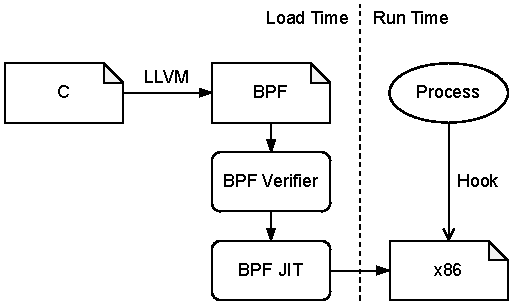
\includegraphics[width=0.6\linewidth]{figures/sec-2-ebpf.pdf}
  \caption{eBPF execution pipeline. C source is compiled to BPF bytecode, verified and JIT-compiled at load time, then executed as native x86 code at runtime via kernel hooks.}
  \label{fig:ebpf}\end{figure}
